\section{Power Management and Monitoring}
\label{sec:power-management}

The Loon-E electrical architecture is designed for high-performance propulsion while maintaining a redundant power supply for critical electronics and emergency recovery.

\subsection{Dual-Battery Switching System}
\label{subsec:battery-switching}

The power system is split into two distinct voltage domains to prevent high-current motor noise from affecting sensitive sensors:
\begin{itemize}
    \item \textbf{Propulsion Supply:} Two 20V, 6Ah Lithium-Ion batteries. These are used to run the T200 thrusters at their maximum potential, providing up to 12.5 kgf of thrust.
    \item \textbf{System Supply:} A single 14.8V, 18Ah battery. This provides a stable power source for the Jetson Orin Nano, ZED X camera, and communications hardware.
\end{itemize}

A core innovation of the Loon-E is the \textbf{Emergency Relay Switch}. A set of high-current relays (30A rated) allows the system to alternate the power source for the propellers. While the propellers run on the 20V batteries by default, they can be switched to the 14.8V system battery. This serves as a fail-safe mechanism, ensuring the vessel can be safely returned to shore under RC control if the primary propulsion batteries are depleted or fail.

\subsection{Voltage Monitoring and Safety}
\label{subsec:voltage-monitoring}

To protect the Lithium-Ion cells and provide real-time telemetry, the system employs three layers of monitoring:

\begin{itemize}
    \item \textbf{BMS Protection:} All batteries are integrated with a Battery Management System (BMS). For the 14.8V battery, the BMS monitors individual cell levels and will automatically cut output if a cell reaches the minimum safe voltage.
    \item \textbf{Custom Voltage Sensors:} The team developed custom PCBs utilizing a voltage divider and an Analog-to-Digital Converter (ADC). These sensors relay voltage data for all three batteries to the Jetson Orin Nano via the I2C protocol, which is then transmitted to the ground station.
    \item \textbf{RC Telemetry:} A secondary voltage sensor is placed at the BMS output to provide direct feedback to the operator's FlySky remote. If the BMS triggers a safety cutoff, the remote display drops to 0V, providing an immediate alert to the pilot.
    \item \textbf{Overcurrent Protection:} The propulsion circuitry includes 285-Series circuit breakers. These are calibrated to trip at 30A, protecting the ESCs and 10 AWG wiring from the maximum allowable operating current (28.26A).
\end{itemize}

\begin{figure}[H]
    \centering
    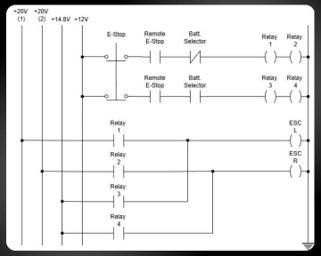
\includegraphics[width=0.8\textwidth]{images/Electronic_Diagram_for_Dual_Battery_System.jpg}
    \caption{Electronic Diagram for Dual Battery System (Ref: Technical Report Fig. 5)}
    \label{fig:dual-battery-schematic}
\end{figure}